\documentclass[11pt]{article}
\input{/Users/markwang/.preamble}
\begin{document}

\newcommand{\calE}{\mathcal{E}}
\newcommand{\calR}{\mathcal{R}}
\newcommand{\calS}{\mathcal{S}}
\newcommand{\calL}{\mathcal{L}}
\newcommand{\lebpar}[2]{\frac{\partial #1}{\partial #2}}

\begin{enumerate}
\item \textbf{Hard-Coding a Network} In this problem, you need to find a set of weights and biases for a multilayer perceptron which determines if a list of length 4 is in sorted order. More specifically, you receive four inputs $x_1,\cdots,x_4$, where $x_i\in \R$, and the network must output 1 if $x_1 < x_2 < x_3 < x_4$, and 0 otherwise. All hidden units and the output unit use a hard threshold activation function
\[
    \phi(z) = 
    \begin{cases}
        1 & z \geq 0 \\ 
        0 & z < 0
    \end{cases}    
\]
\begin{solution}
    We will set weight and biases such that $h_j$ activates if $x_j < x_{j+1}$. For example, we want $h_1 = 1$ if $x_1 < x_2$, that is for
    \[
        w_{11} x_1 + w_{12} x_2 + w_{13} x_3 + w_{14} x_4 + b_1> 0
    \]
    weights $(1, -1, 0, 0)$ and bias of $-0.1$ satisfies the constraint. Similarly, we can hard code weights and biases for $h_2$ and $h_3$. 
    \[
        \mathbf{W}^{(-1)} = 
        \begin{pmatrix}
            1 & -1 & 0 & 0 \\
            0 & 1 & -1 & 0 \\
            0 & 0 & 1 & -1 \\ 
        \end{pmatrix} 
        \quad \quad \quad 
        \mathbf{b}^{(1)} = 
        \begin{pmatrix}
            0\\ 0 \\ 0 \\
        \end{pmatrix}
    \]
    Now we set weights and bias for computing $y$ such that $y$ activates if and only if all $h_1,h_2,h_3$ activates 
    \[
        \mathbf{w}^{(2)} = 
        \begin{pmatrix}
            -10 & -10 & -10 \\ 
        \end{pmatrix}
        \quad \quad \quad 
        b^{(2)} = 0.5
    \]

\end{solution}

\item \textbf{Backprop} Consider a neural network with $N$ input units, $N$ output units, and $K$ hidden units. The activations are computed as follows: 
\begin{align*}
    \matr{z} &= \matr{W^{(1)}x + b^{(1)}} \\
    \matr{h} &= \sigma(\matr{z}) \\
    \matr{y} &= \matr{x + W^{(2)}h + b^{(2)}} \\ 
\end{align*}
The cost involves both $\matr{h}$ and $\matr{y}$ 
\begin{align*}
    \calE &= \calR + \calS \\
    \calR &= \matr{r^T h} \\
    \calS &= \frac{1}{2} ||\matr{y-s}||^2 \\ 
\end{align*}
for given vector $\matr{r}$ and $\matr{s}$
\begin{enumerate}
    \item Draw computation graph 
    \begin{center}
        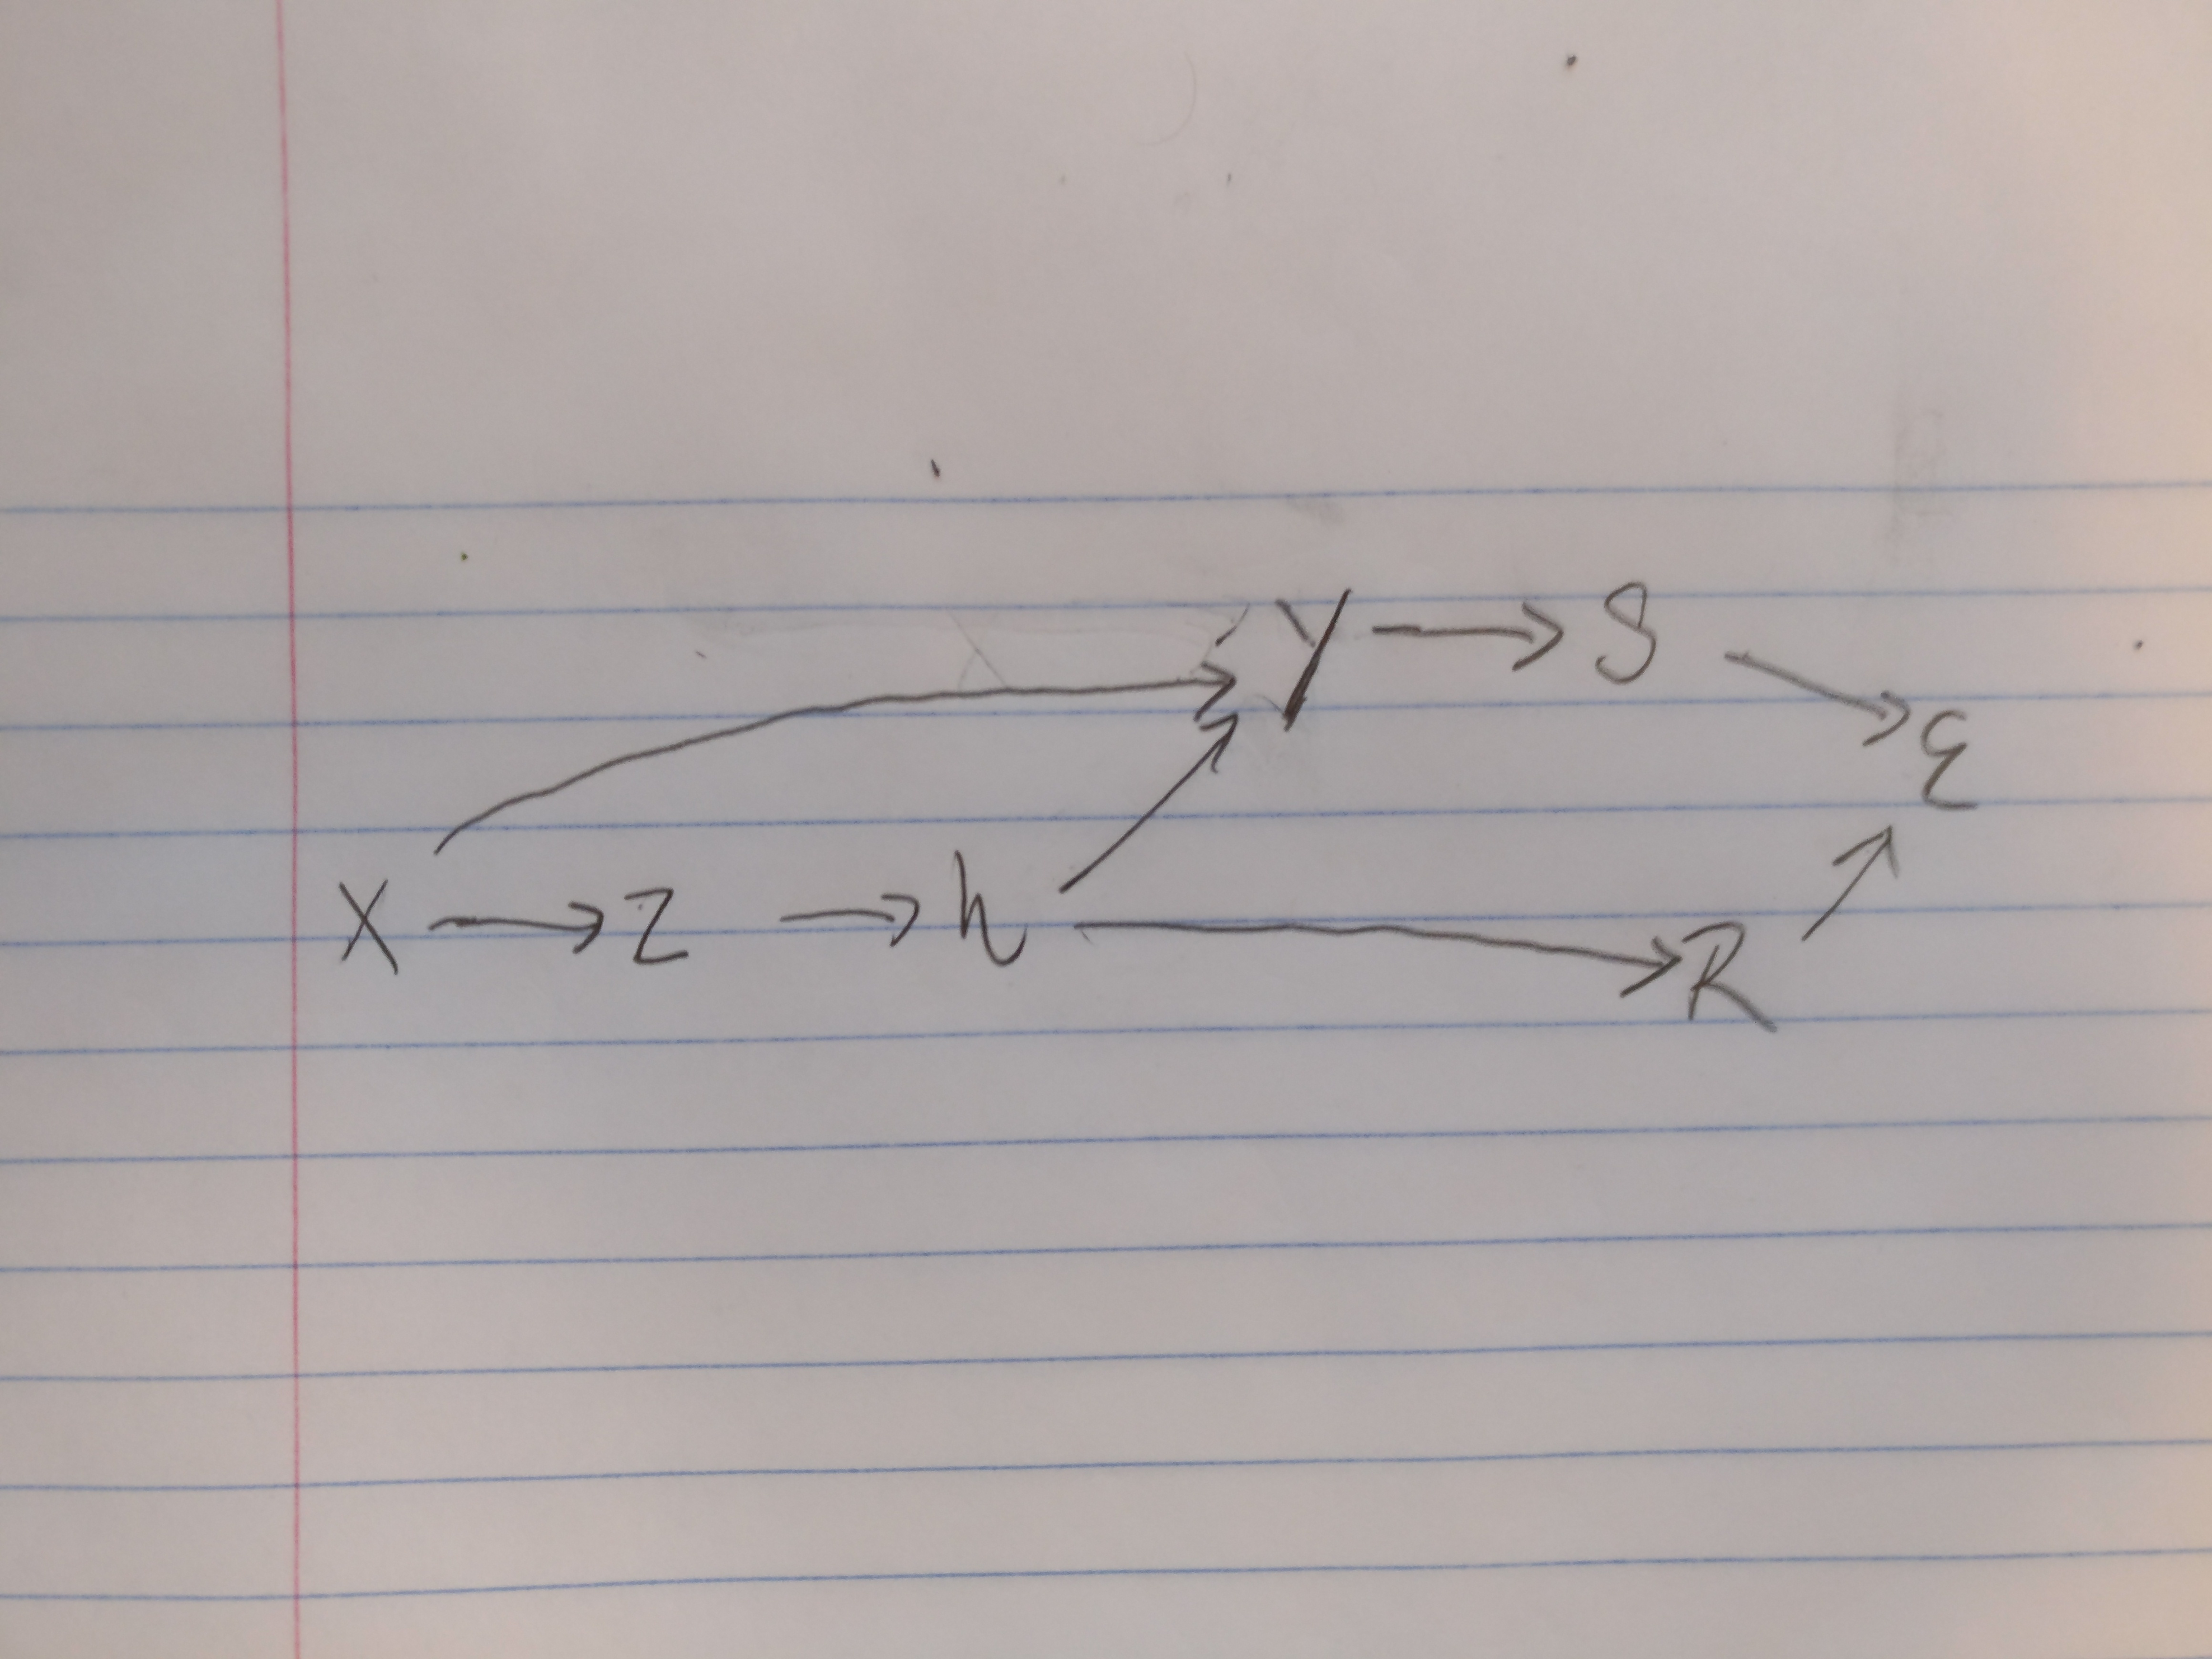
\includegraphics[width=7cm]{computation_graph.jpg}
    \end{center}
    \item Derive backprop equations for computing $\overline{x} = \rfrac{\partial \calE}{\partial \matr{x}}$ 
    \begin{solution}
        We first derive scalar form for the forward pass 
        \begin{align*}
            \calE &= \calR + \calS \\ 
            \calS &= \frac{1}{2} \sum_{i=1}^N (y_i - s_i)^2 \\
            \calR &= \sum_{j=1}^K r_j h_j \\
            y_i   &= x_i + \sum_j^K w_{ij}^{(2)} h_j + b_i^{(2)} \\  
            h_j   &= \sigma(z_j) \\
            z_j   &= \sum_{i=1}^N w_{ji}^{(1)} x_i + b_j^{(1)} \\
        \end{align*}
        for $i=1,2,\dots, N$ and $j=1,2,\cdots, K$. Then we derive the scalar form for the reverse pass, 
        \begin{align*}
            \bar{\calE} &= 1 \\
            \bar{\calR} &= \bar{\calE} \lebpar{\calE}{\calR} = 1 \\ 
            \bar{\calS} &= \bar{\calE} \lebpar{\calR}{\calS} = 1 \\
            \bar{y}_i   &= \bar{\calS} \lebpar{\calS}{y_i} = y_i - s_i \\ 
            \bar{h}_j   &= \bar{\calR} \lebpar{\calR}{h_j} + \sum_{i=1}^N \bar{y}_i \lebpar{y_i}{h_j} = r_j + \sum_{i=1}^N \bar{y}_i w_{ij}^{(2)} \\
            \bar{z}_j   &= \bar{h}_j \lebpar{h_j}{z_j} = \bar{h}_j \sigma'(z_j) \\
            \bar{x}_i   &= \sum_{j=1}^K \bar{z}_j \lebpar{z_j}{x_i} + \bar{y}_i \lebpar{y_i}{x_i} = \sum_{j=1}^K \bar{z}_j w_{ji}^{(1)} + \bar{y}_i
        \end{align*}
        Then vectorize the result 
        \begin{align*}
            \bar{\calE} &= 1\\
            \bar{\calR} &= 1\\
            \bar{\calE} &= 1 \\
            \matr{\bar{y}} &= \matr{y-s} \\
            \matr{\bar{h}} &= \matr{r + W^{(2)T} \bar{y}} \\
            \matr{\bar{z}} &= \matr{\bar{h}} \circ \sigma'(\matr{z}) \\ 
            \matr{\bar{x}} &=  \matr{W^{(1)T} \bar{z} + \bar{y}} \\ 
        \end{align*}
    \end{solution}
\end{enumerate}

\item \textbf{Sparsifying Activation Function} 
\begin{solution}
    \begin{align*}
        \lebpar{\calL}{w_1} \quad \quad \text{YES} \\ 
        \lebpar{\calL}{w_2} \quad \quad \text{YES} \\ 
        \lebpar{\calL}{w_3} \quad \quad \text{NO} \\ 
    \end{align*}
    If $h_1$ is 0, then $y$ do not depend on $w_1h_1 = 0$ and so the a measure in change of $\calL$ with respect to $w_1$ while holding other variables constant is zero, i.e. $\lebpar{\calL}{w_1} = 0$. A infinitesimal change in $w_2$ yields negative value as input to $h_1$, by similar argument shown previously, we have $\lebpar{\calL}{w_2} = 0$. However, a small change in $w_3$ might result in changes in $y$ if both $h_2, h_3$ activates, and so $\lebpar{\calL}{w_3}$ might not be zero.
    
\end{solution}






\end{enumerate}






\end{document}
